%\chapter{spacereq}

%%%%%%%%%%%%%%%%%%%%%%%%%%%%%%%%%%%%%%%%%%%%%%
\section{Installation space and clean room}

ProtoDUNE-SP will be housed in an extension to the EHN1 hall in the North Area of the Pr\'{e}vessin site at CERN. 
The cryostat will be constructed in a pit inside the building and will be surrounded on three sides by the pit walls.  On the open side of the cryostat will be an ISO 8 clean room that will be used to construct, test and assemble the TPC. A material pass-through structure (material SAS) will be adjacent to the clean room. Figure~\ref{fig:cryostat-in-ehn1} shows the layout of these structures in EHN1. 
\fixme{define SAS}

Material will be brought into EHN1, passed down into the SAS through its removable roof, then transported through a set of large doors from the SAS into the clean room where it will be tested and assembled. When ready, each assembled TPC component will pass through a temporary construction opening (TCO) in the cryostat for installation.
While material is lowered into the SAS from the gallery floor, the doors to the clean room will remain closed to reduce contamination of the clean room space.
Once the roof of the SAS is closed, these doors can be opened to move the material into the clean room.  

In addition to filtering the air in the clean room, the lighting inside it and any temporary lighting inside the cryostat will be filtered to limit the exposure of the PDS components to UV light.  Wavelengths below 450~nm will be filtered out.   

\begin{cdrfigure}[ProtoDUNE-SP cryostat in EHN1]{cryostat-in-ehn1}{Layout of ProtoDUNE-SP cryostat, clean room and material SAS in EHN1}
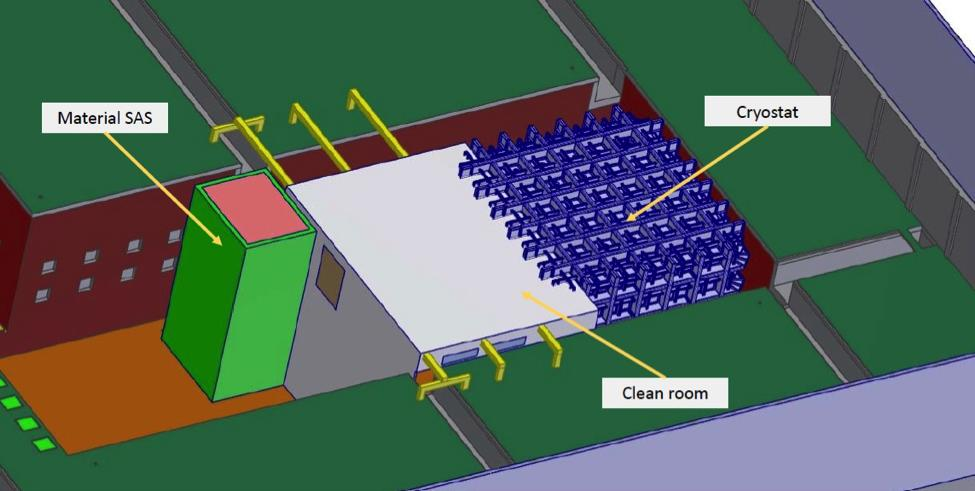
\includegraphics[width=0.8\textwidth]{sp-cryostat-in-ehn1}
\end{cdrfigure}

A naming convention has been established to label the four sides of the cryostat for logistical purposes, shown in Figure~\ref{fig:cryo-side-names}.  The upper side is \textit{Jura}, the lower is \textit{Sal\`{e}ve}, the left is \textit{Beam}, and right is \textit{Downstream}.

\begin{cdrfigure}[Conventions for labeling the four sides of the cryostat]{cryo-side-names}{Conventions for labeling the four sides of the cryostat}
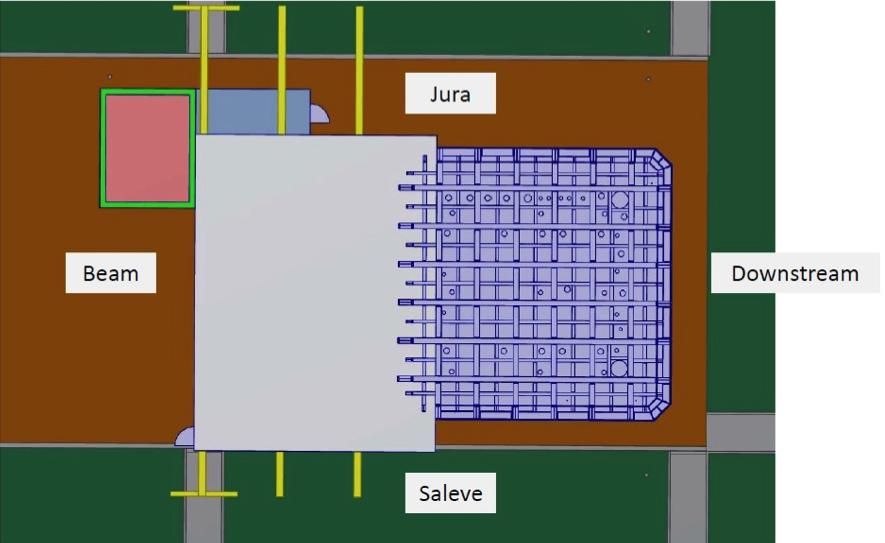
\includegraphics[width=0.8\textwidth]{naming-conv-cryo-sides}
\end{cdrfigure}

Figure~\ref{fig:elev-view-cryostat} is an elevation section view of the cryostat that shows the position of the TCO and the location of the integrated cold testing stand that will be described in Section~\ref{sec:quality:space}.  

\begin{cdrfigure}[Elevation section view of the cryostat]{elev-view-cryostat}{Elevation section view of the cryostat}
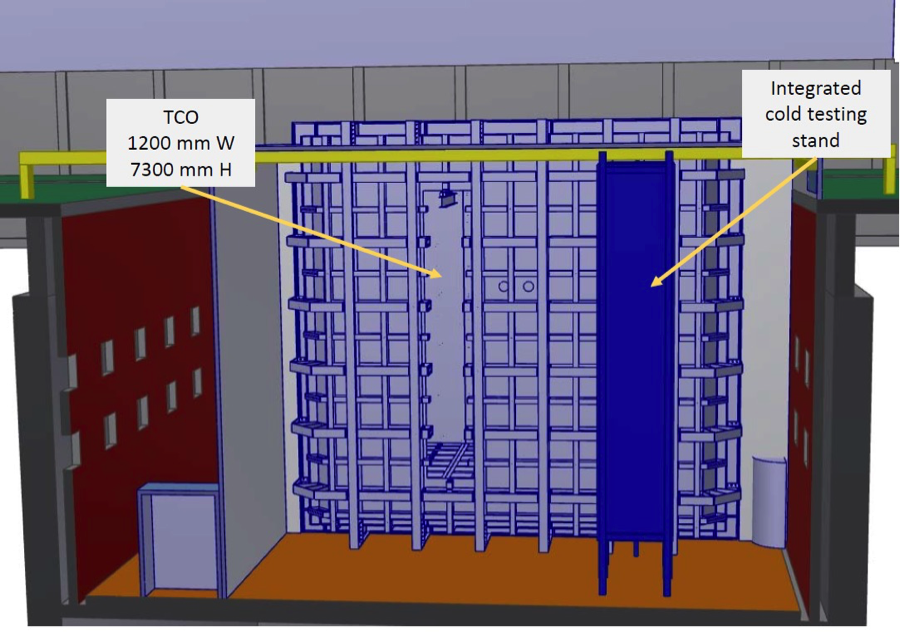
\includegraphics[width=0.8\textwidth]{elev-view-cryostat}
\end{cdrfigure}

Inside the clean room, a series of rails will facilitate the movement of the TPC components during the test and installation processes.  The conceptual layout of these rails is shown in Figure~\ref{fig:rails-in-cleanroom}.  The rails will be positioned vertically at the same height of the DSS rails inside the cryostat.  A temporary rail will be installed through the TCO that bridges the DSS and the rails in the clean room.  All of the large components of the cryogenic piping and TPC will be supported from these rails on movable trolleys as they are transported to the interior of the cryostat.  

\begin{cdrfigure}[Layout of rails in clean room and dimensions]{rails-in-cleanroom}{Conceptual layout of rails in clean room to facilitate movement of TPC components; approximate dimensions for the material SAS and the footprint of the clean room space are shown.}
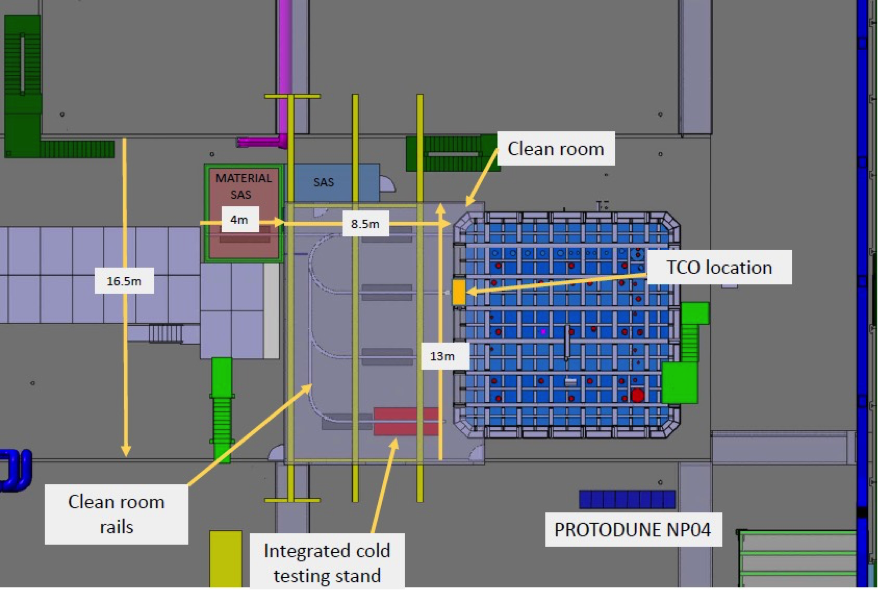
\includegraphics[width=0.8\textwidth]{rails-in-cleanroom}
\end{cdrfigure}


Figure~\ref{fig:rails-in-cleanroom} also shows the approximate dimensions for the Material SAS and the footprint of the clean room space.  This space is 
\fixme{these spaces are?} limited by the pit walls on two sides (top and bottom of figure), and by the supports for the beam and beam instrumentation on the other  (left side of figure).  

Figure~\ref{fig:sas-locations} shows the planned locations for all of the activities that will be performed inside the clean room.  

\begin{cdrfigure}[Locations of activities in clean room]{sas-locations}{Locations of activities to be performed in the clean room}
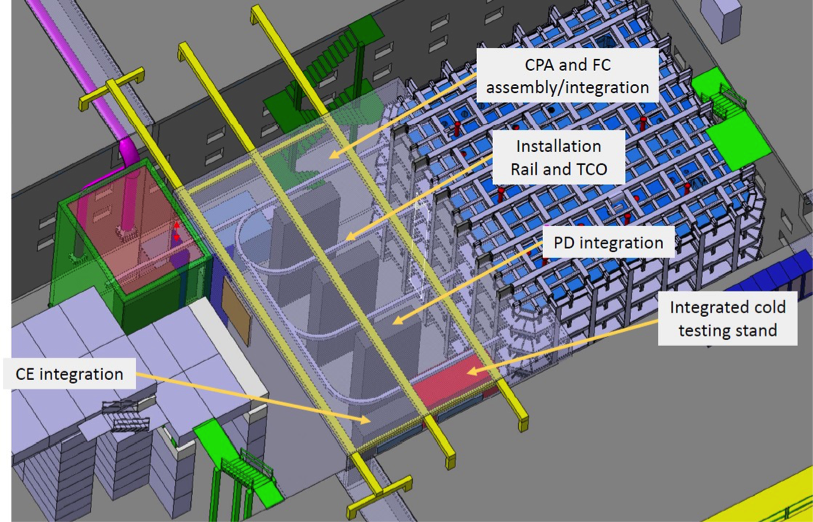
\includegraphics[width=0.8\textwidth]{sas-locations}
\end{cdrfigure}

The activities that will take place in the clean room include:
\begin{itemize}
\item Assembly of the CPA panels into CPA modules on a large horizontal surface.
%.  This requires a large flat surface approximately 1500 mm $\times$ 6500 mm 
%to join the three CPA panels into one CPA module.  Once these are assembled, an overhead hoist located near the TCO will be used to translate the CPA module from horizontal to vertical and place it for attachment to the clean room rails.  
\item Rotation of CPA modules from horizontal to vertical, and placement on the clean room rails.  
%\item Attachment of the upper and lower FC assemblies to the CPA modules.  Once two of the CPA modules are attached to the clean room rail, two upper and two lower FC assemblies will be attached.  This will be done with the same overhead hoist located near the TCO.
\item Attachment of FC assemblies to CPA modules.
\item Unpacking and testing of the PDS elements, and installation of them on the APA frames.  
\item Unpacking and testing of the CE  elements, and mounting of the CE onto the APAs.   
\item Integrated testing of APA with PDS and CE.  
\end{itemize}

